\documentclass[border={0.5cm 0.5cm 0.5cm 0.5cm}]{standalone}

\usepackage{amssymb}
\usepackage{amsmath}
\usepackage{tikz}
\usetikzlibrary{calc}					%for centerarc
\usetikzlibrary{arrows, arrows.meta}	%for big arrowheads

\def\centerarc[#1](#2)(#3:#4:#5)% Syntax: [draw options] (center) (initial angle:final angle:radius)
{ \draw[#1] ($(#2)+({#5*cos(#3)},{#5*sin(#3)})$) arc (#3:#4:#5); }

%The social in a dynamic diagram (Albertsen & Diken, 2006: 239)
%Albertsen, N. & Diken, B. (2006). “Society with/out organs,” in Fuglsang, M. & Sørensen, B.
%(2006). Deleuze and the social. Edinburgh: Edinburgh University Press, p. 239 (fig. 12.1)

\begin{document}
	
	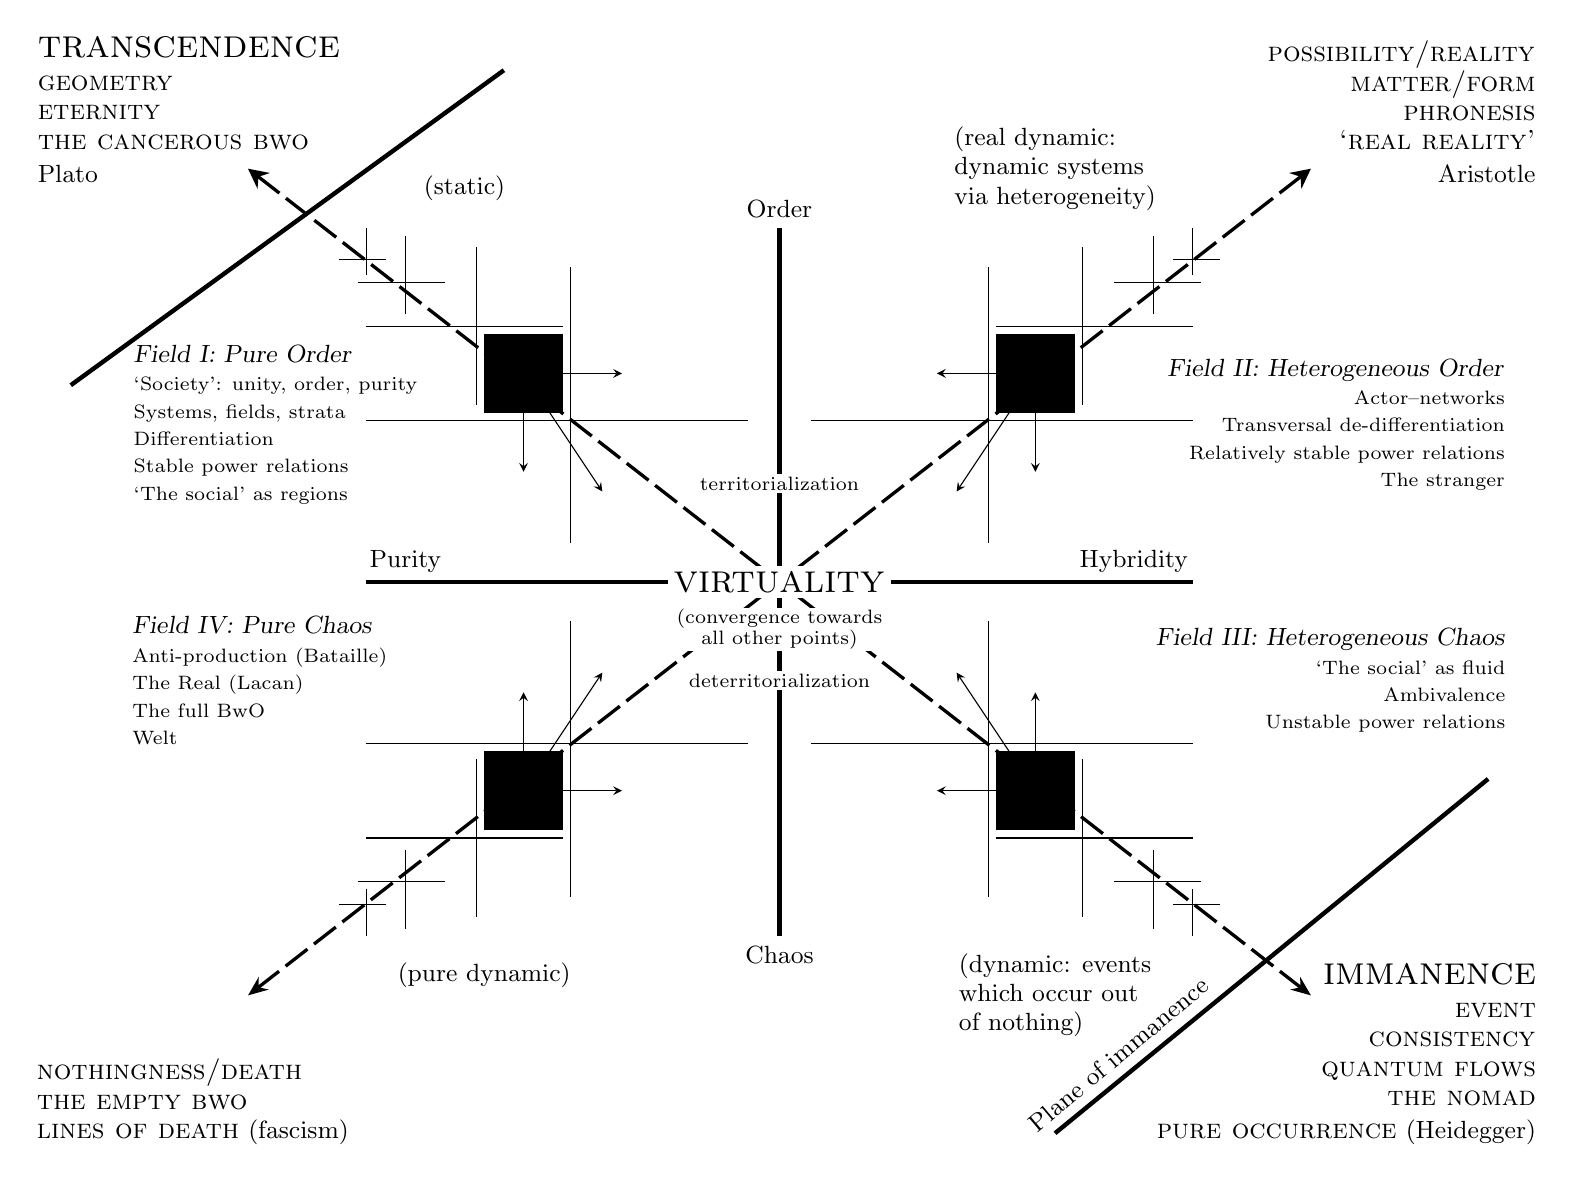
\begin{tikzpicture}
	%AXIS
	\draw[ultra thick] (-5.25,0)--(5.25,0);	%horizontal
	\draw[ultra thick] (0,-4.5)--(0,4.5);	%vertical
	\draw[ultra thick] (-9,2.5)--(-3.5,6.5); %top-left
	\draw[ultra thick] (9,-2.5)--(3.5,-7); %bottom-right
	\node at (4.3,-6) {\rotatebox{40}{\small Plane of immanence}};
	\draw[very thick,{Stealth[length=2.5mm,width=2.5mm]}-{Stealth[length=2.5mm,width=2mm]},
	dashed,dash pattern=on 10pt off 3pt] (-6.75,5.25)--(6.75,-5.25);
	\draw[very thick,{Stealth[length=2.5mm,width=2.5mm]}-{Stealth[length=2.5mm,width=2mm]},
	dashed,dash pattern=on 10pt off 3pt] (6.75,5.25)--(-6.75,-5.25);
	\centerarc[{Stealth[length=2.5mm,width=2mm]}-{Stealth[length=2.5mm,width=2mm]},semithick](0,0)(-139:139:1.9)
	
	%SQUARES
	\fill (-3.25-0.5,-2.65-0.5) rectangle (-3.25+0.5,-2.65+0.5);
		\draw[->,>=stealth] (-3.25,-2.65)--++(0,1.25);
		\draw[->,>=stealth] (-3.25,-2.65)--++(1.25,0);
		\draw[->,>=stealth] (-3.25,-2.65)--++(1,1.5);
	\fill (-3.25-0.5,2.65-0.5) rectangle (-3.25+0.5,2.65+0.5);
		\draw[->,>=stealth] (-3.25,2.65)--++(0,-1.25);
		\draw[->,>=stealth] (-3.25,2.65)--++(1.25,0);
		\draw[->,>=stealth] (-3.25,2.65)--++(1,-1.5);
	\fill (3.25-0.5,-2.65-0.5) rectangle (3.25+0.5,-2.65+0.5);
		\draw[->,>=stealth] (3.25,-2.65)--++(0,1.25);
		\draw[->,>=stealth] (3.25,-2.65)--++(-1.25,0);
		\draw[->,>=stealth] (3.25,-2.65)--++(-1,1.5);
	\fill (3.25-0.5,2.65-0.5) rectangle (3.25+0.5,2.65+0.5);
		\draw[->,>=stealth] (3.25,2.65)--++(0,-1.25);
		\draw[->,>=stealth] (3.25,2.65)--++(-1.25,0);
		\draw[->,>=stealth] (3.25,2.65)--++(-1,-1.5);
	
	%CROSSES
	%bottom-left
	\draw (-0.4,-2.05)--(-5.25,-2.05);  %--, big
	\draw (-2.65,-0.5)--(-2.65,-4.00);  %|, big
	\draw (-5.25,-3.25)--(-2.75,-3.25); %--, medium
	\draw (-3.85,-2.25)--(-3.85,-4.25); %|, medium
	\draw (-5.35,-3.8)--(-4.25,-3.8);	%--, small
	\draw (-4.75,-3.4)--(-4.75,-4.4);	%|, small
	\draw (-5.6,-4.1)--(-5.0,-4.1);		%--, tiny
	\draw (-5.25,-3.9)--(-5.25,-4.5);	%|, tiny
	%bottom-right
	\draw (0.4,-2.05)--(5.25,-2.05);	%--, big
	\draw (2.65,-0.5)--(2.65,-4.00);	%|, big
	\draw (5.25,-3.25)--(2.75,-3.25);	%--, medium
	\draw (3.85,-2.25)--(3.85,-4.25);	%|, medium
	\draw (5.35,-3.8)--(4.25,-3.8);		%--, small
	\draw (4.75,-3.4)--(4.75,-4.4);		%|, small
	\draw (5.6,-4.1)--(5.0,-4.1);		%--, tiny
	\draw (5.25,-3.9)--(5.25,-4.5);		%|, tiny
	%top-left
	\draw (-0.4,2.05)--(-5.25,2.05);	%--, big
	\draw (-2.65,0.5)--(-2.65,4.00);	%|, big
	\draw (-5.25,3.25)--(-2.75,3.25);	%--, medium
	\draw (-3.85,2.25)--(-3.85,4.25);	%|, medium
	\draw (-5.35,3.8)--(-4.25,3.8);		%--, small
	\draw (-4.75,3.4)--(-4.75,4.4);		%|, small
	\draw (-5.6,4.1)--(-5.0,4.1);		%--, tiny
	\draw (-5.25,3.9)--(-5.25,4.5);		%|, tiny
	%top-right
	\draw (0.4,2.05)--(5.25,2.05);		%--, big
	\draw (2.65,0.5)--(2.65,4.00);		%|, big
	\draw (5.25,3.25)--(2.75,3.25);		%--, medium
	\draw (3.85,2.25)--(3.85,4.25);		%|, medium
	\draw (5.35,3.8)--(4.25,3.8);		%--, small
	\draw (4.75,3.4)--(4.75,4.4);		%|, small
	\draw (5.6,4.1)--(5.0,4.1);			%--, tiny
	\draw (5.25,3.9)--(5.25,4.5);		%|, tiny
	
	%LABELS -- AXIS
	\node[above] at (-4.75,0) {\small Purity};
	\node[above] at (4.5,0) {\small Hybridity};
	\node[above] at (0,4.5) {\small Order};
	\node[below] at (0,-4.5) {\small Chaos};
	\node[fill=white,inner sep=1] at (0,1.25) {\scriptsize territorialization};
	\node[fill=white,inner sep=1] at (0,-1.25) {\scriptsize deterritorialization};
	\node[fill=white,inner sep=2] at (0,0) {\textsc{\Large virtuality}};
	\node[align=center,fill=white,inner sep=0.5] at (0,-0.6) 
	{\scriptsize (convergence towards\\[-1.5mm]\scriptsize all other points)};
	
	%LABELS -- OUTER
	\node[align=left] at (-7.5,6) {\textsc{\Large transcendence}\\
								   \textsc{geometry}\\[-0.5mm]
								   \textsc{eternity}\\[-0.5mm]
								   \textsc{the cancerous bwo}\\
								   {\small Plato}
								  };
	\node[align=right] at (7.9,5.97) {\textsc{possibility/reality}\\[-0.5mm]
									  \textsc{matter/form}\\[-0.5mm]
									  \textsc{phronesis}\\[-0.5mm]
									  \textsc{`real reality'}\\
									 {\small Aristotle}
								     };
	\node[align=left] at (-7.45,-6.6) {\textsc{nothingness/death}\\[-0.5mm]
									 \textsc{the empty bwo}\\[-0.5mm]
									 \textsc{lines of death} {\small(fascism)}
									 };
	\node[align=right] at (7.2,-6) {\textsc{\Large immanence}\\
								    \textsc{event}\\[-0.5mm]
								    \textsc{consistency}\\[-0.5mm]
								    \textsc{quantum flows}\\[-0.5mm]
								    \textsc{the nomad}\\
								    \textsc{pure occurrence} {\small (Heidegger)}
								   };
	
	%LABELS -- INNER
	\node[align=left] at (-6.4,2) {\textsl{\small Field I: Pure Order}\\[-0.6mm]
		{\scriptsize `Society': unity, order, purity}\\[-0.75mm]
		{\scriptsize Systems, fields, strata}\\[-0.75mm]
		{\scriptsize Differentiation}\\[-0.75mm]
		{\scriptsize Stable power relations}\\[-0.75mm]
		{\scriptsize `The social' as regions}
	};
	\node[align=right] at (7.07,2) {\textsl{\small Field II: Heterogeneous Order}\\[-0.6mm]
		{\scriptsize Actor--networks}\\[-0.75mm]
		{\scriptsize Transversal de-differentiation}\\[-0.75mm]
		{\scriptsize Relatively stable power relations}\\[-0.75mm]
		{\scriptsize The stranger}
	};
	\node[align=right] at (7,-1.25) {\textsl{\small Field III: Heterogeneous Chaos}\\[-0.6mm]
		{\scriptsize `The social' as fluid}\\[-0.75mm]
		{\scriptsize Ambivalence}\\[-0.75mm]
		{\scriptsize Unstable power relations}
	};
	\node[align=left] at (-6.6,-1.25) {\textsl{\small Field IV: Pure Chaos}\\[-0.6mm]
		{\scriptsize Anti-production (Bataille)}\\[-0.75mm]
		{\scriptsize The Real (Lacan)}\\[-0.75mm]
		{\scriptsize The full BwO}\\[-0.75mm]
		{\scriptsize Welt}
	};
	\node at (-4,5) {\small (static)};
	\node at (-3.75,-5) {\small (pure dynamic)};
	%\node[align=left] at (3.5,5.25) {\small (real dynamic:\\\small dynamic systems\\\small by virtue of\\\small heterogeneity)};
	\node[align=left] at (3.5,5.25) {\small (real dynamic:\\[-0.5mm]\small dynamic systems\\[-0.5mm]\small via heterogeneity)};
	\node[align=left] at (3.5,-5.25) {\small (dynamic: events\\[-0.5mm]\small which occur out\\[-0.5mm]\small of nothing)};
	\end{tikzpicture}
	
\end{document}